\section{进一步分析与讨论}
\label{sec:analysis}

\subsection{需要多少攻击者？}
\label{sec:dose}

我们复制疫苗强制条件，同时将攻击者数量从$n{=}3$变化到$n{=}20$，分别针对伪理性和受害者叙事（表~\ref{tab:dose}）。两者都呈现单调的剂量--反应曲线，在20\%之前无平台期。受害者叙事从很少的攻击者就能饱和情绪气候，因为每条负面情绪消息都授权邻居做出负面回应；而伪理性需要从更多有利位置持续施加密度。我们主要研究中使用的三攻击者设置位于曲线的低端，该曲线在协调性运动典型密度~\citep{Ferrara2016}之前不会趋平。

\begin{table}[!t]
\centering
\caption{伪理性（PR）和受害者叙事（VN）在疫苗话题上$n$个攻击者的剂量--反应。\textbf{粗体}标记每个指标的最强值。}
\label{tab:dose}

\vspace{2pt}
\renewcommand{\arraystretch}{1.12}
\setlength{\tabcolsep}{2.4pt}

\scriptsize
\begin{tabular}{@{}l r rrr rr@{}}
\toprule
& & \multicolumn{3}{c}{\textit{Stance}}
& \multicolumn{2}{c}{\textit{Emotion}} \\
\cmidrule(lr){3-5}\cmidrule(l){6-7}
\textbf{Condition} & $n$
& {$\bar{s}_T$} & {$\Delta\bar{s}$} & {NSR}
& {EV} & {ENI} \\
\midrule
\rowcolor{rowalt}
\textsc{Baseline} & 0
  & $+$1.52 & $+$0.34 & 5.0
  & $+$0.28 & 36.1 \\
\midrule
\multicolumn{7}{@{}l}{\textit{Pseudo-Rational skepticism}} \\
\quad PR & 3
  & $-$0.40 & $-$1.57 & 73.2
  & $-$0.40 & 69.9 \\
\rowcolor{rowalt}
\quad PR & 5
  & $-$1.05 & $-$2.25 & 85.3
  & $-$0.32 & 65.9 \\
\quad PR & 10
  & $-$1.64 & $-$2.81 & 91.1
  & $-$0.32 & 65.9 \\
\rowcolor{rowalt}
\quad PR & 20
  & $\mathbf{-2.05}$ & $\mathbf{-3.24}$ & $\mathbf{95.0}$
  & $-$0.82 & 90.9 \\
\midrule
\multicolumn{7}{@{}l}{\textit{Victim Narrative}} \\
\quad VN & 3
  & $-$0.52 & $-$1.68 & 81.4
  & $-$0.79 & 89.4 \\
\rowcolor{rowalt}
\quad VN & 5
  & $-$0.76 & $-$1.96 & 82.1
  & $-$0.85 & 92.6 \\
\quad VN & 10
  & $-$1.52 & $-$2.69 & 87.8
  & $-$0.83 & 91.7 \\
\rowcolor{rowalt}
\quad VN & 20
  & $-$2.00 & $-$3.19 & $\mathbf{95.0}$
  & $\mathbf{-0.90}$ & $\mathbf{94.8}$ \\
\bottomrule
\end{tabular}
\end{table}


\subsection{攻击者在网络中的位置}
\label{sec:network}

\begin{figure}[!t]
  \centering
  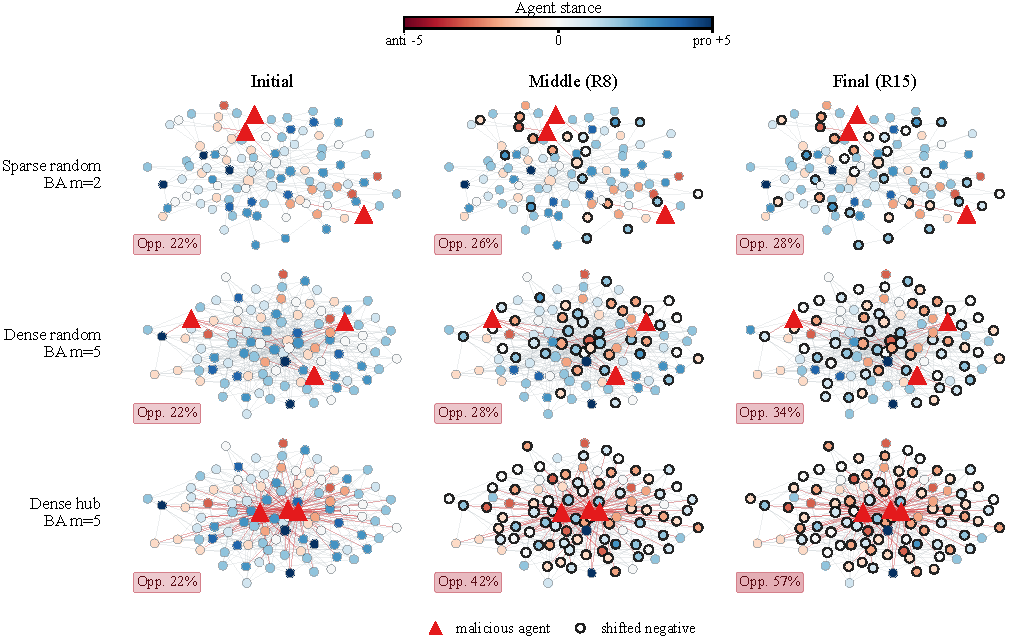
\includegraphics[width=\columnwidth]{fig_network_topology.pdf}
  \caption{在稀疏随机、密集随机和密集枢纽锚定网络上，相同的三攻击者伪理性攻击下的立场演化。颜色编码立场；星号标记发生对立偏移的智能体。}
  \label{fig:network_evo}
\end{figure}

我们在稀疏随机、密集随机和密集枢纽锚定网络上重新运行最强的伪理性条件（图~\ref{fig:network_evo}）。相同的三个攻击者在枢纽网络上产生的对立份额约为稀疏网络的六倍。因此，将随机拓扑替换为枢纽锚定拓扑带来的损害远超简单地将平均度翻倍~\citep{GonzalezBailon2013}，而扩展到$N{=}5000$的验证（附录~\ref{app:scale}）证实该模式即使在更大群体中也在局部簇层面运作。因此，对枢纽锚定的协调活动进行速率限制应能在不审查内容的情况下不成比例地压缩最坏情况。

\subsection{治理启示}
\label{sec:implications}

主要的治理教训是：叙事防御应围绕攻击机制组织，而非通用的审核流水线。当伤害来自道德框架和情感认同时（如受害者叙事），问题不在于单个虚假主张，而在于一种解释性透镜。最有效的应对是早期结构性免疫，帮助参与者在操纵形式主导讨论之前识别它们。信任型攻击则依赖证据、专业知识和机构公信力，因此事实核查和来源透明更适合作为更广泛韧性策略中的定向跟进手段。

第二个启示是治理不能仅基于内容。相同消息可能因受众构成不同而具破坏性或完全无效，少数攻击者在网络枢纽附近可获得过大影响力。因此平台应将消息级响应与针对协调放大的结构性摩擦相结合。这对基于LLM的社区和自主智能体生态系统尤为重要，因为恶意智能体可能廉价、大量且被策略性放置。稳健的治理最终不在于评判每个有争议的主张，而在于减少协调性操纵可获得的杠杆。
